\documentclass{article}

\usepackage{dirtree}

\usepackage[
  height=9in,      % height of the text block
  width=7.5in,       % width of the text block
  top=78pt,        % distance of the text block from the top of the page
  headheight=48pt, % height for the header block
  headsep=12pt,    % distance from the header block to the text block
  heightrounded,   % ensure an integer number of lines
        % show the main blocks
  verbose,         % show the values of the parameters in the log file
]{geometry}
\setlength{\parindent}{0pt}
\usepackage{amsmath}
\usepackage{courier}
\usepackage{graphicx}
\usepackage{amsmath}
\usepackage{booktabs}
\usepackage{fancyhdr}
\usepackage{float}
\usepackage{mathtools}

\pagestyle{fancy}
\fancyhead[L]{Pattern and Speech Recognition WS1617\\ Assignment 04}
\fancyhead[R]{ Vinh Thinh Ho (2562630) \\ Noshaba Cheema (2562653)}



\renewcommand{\headrulewidth}{0.4pt}
\newcommand\tab[1][1cm]{\hspace*{#1}}

\begin{document}
\section*{1) k-Means Clustering}
a) The data:
\begin{figure}[H]
	\centering
	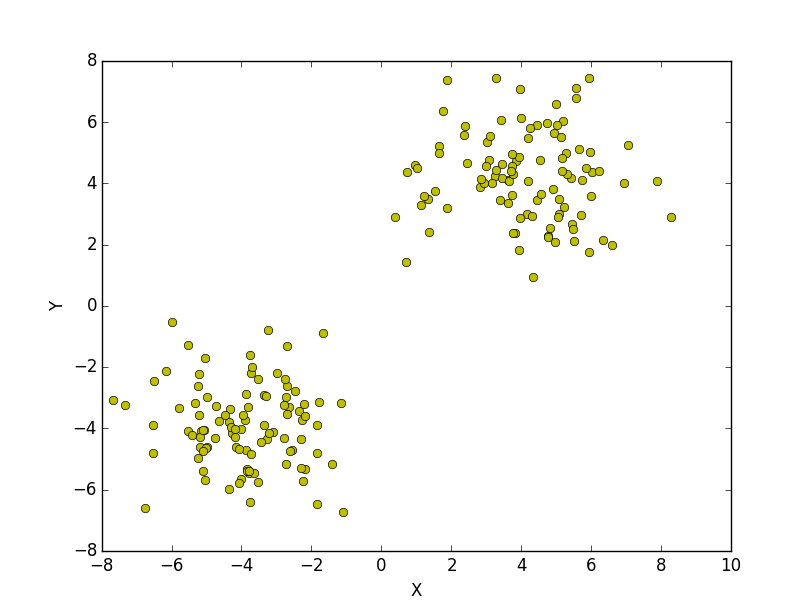
\includegraphics[scale=0.5]{data.png}
	\caption{Data points}
	\label{fig1}	
\end{figure}
b) Implementation of K-means (see \textbf{k-means.py}):\\
c) The clusters:
\begin{figure}[H]
	\centering
	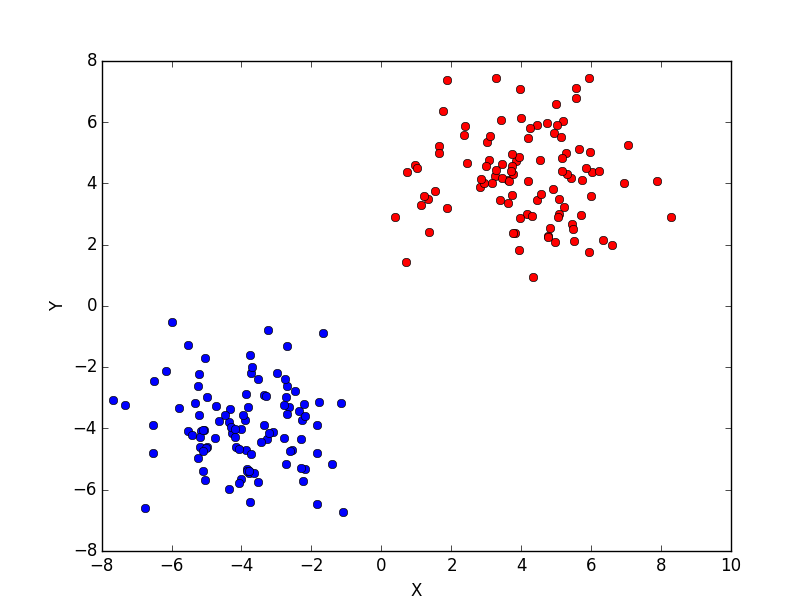
\includegraphics[scale=0.5]{clustered.png}
	\caption{Cluters}
	\label{fig1}	
\end{figure}
d) To get a loss function equals to zero, the distance of each data point to its mean must be equal to zero. In particular, the data point is exactly the same as its mean. So, the number k is at least equal to number of \textbf{distinct} data points.

\section*{2) Maximum Likelihood Estimation}
We have trained data: 
\begin{align*}
K = \{2, 3, 0, 2, 1, 5\}
\end{align*}
We need to maximize the likelihood of trained data:
\begin{align*}
& \max \prod\limits_i \frac{\lambda^{k_i}e^{-\lambda}}{k_i !}\\
\equiv \ & \max \prod\limits_i \lambda^{k_i}e^{-\lambda}\\
\equiv \ & \max \lambda^{\sum\limits_i k_i}e^{-\lambda |K|}\\
\equiv \ & \max \lambda^{13}e^{-6\lambda}\\
\end{align*}
Take the derivative:
\begin{align*}
(\lambda^{13}e^{-6\lambda})' &= (13\lambda^{12}e^{-6\lambda}) + (\lambda^{13}(-6)e^{-6\lambda})\\
&= (\lambda^{12}e^{-6\lambda})(13 - 6\lambda)
\end{align*}
Let the derivative be zero:
\begin{align*}
(\lambda^{12}e^{-6\lambda})(13 - 6\lambda) = 0 \iff \lambda = 0\ OR\ \lambda = \frac{13}{6}
\end{align*}
Because $\lambda$ could not be zero, so we have $\lambda = \frac{13}{6}$

\section*{3) Composite functions}
\begin{align*}
f(x, y) = log(sin(xy)) 
\end{align*}
First order derivative with respect to x:
\begin{align*}
\frac{\partial f}{\partial x} &= \frac{\partial (log(sin(xy)) )}{\partial x}\\
&= \frac{1}{sin(xy)} \frac{\partial (sin(xy))}{\partial x}\\
&= \frac{1}{sin(xy)} cos(xy) \frac{\partial (xy)}{\partial x}\\
&= y\frac{cos(xy)}{sin(xy)} = y\cot(xy)
\end{align*}
The same, we have first order derivative with respect to y:
\begin{align*}
\frac{\partial f}{\partial y} &= x\cot(xy)
\end{align*}
Second order partial derivative with respect to x and y:
\begin{align*}
\frac{\partial^2 f}{\partial xy} = \frac{\partial^2 f}{\partial yx} &=  \frac{\partial(y\cot(xy))}{\partial y}\\
&=cot(xy)\frac{\partial y}{\partial y} + y\frac{\partial(cot(xy))}{\partial y}\\
&= cot(xy) + y(-\frac{x}{sin^2(xy)}) = cot(xy) - \frac{xy}{sin^2(xy)}
\end{align*}
Second order partial derivative with respect to x:
\begin{align*}
\frac{\partial^2 f}{\partial x^2} &=  \frac{\partial(y\cot(xy))}{\partial x}\\
&=cot(xy)\frac{\partial y}{\partial x} + y\frac{\partial(cot(xy))}{\partial x}\\
&= y(-\frac{y}{sin^2(xy)}) = - \frac{y^2}{sin^2(xy)}
\end{align*}
The same, we have second order partial derivative with respect to y:
\begin{align*}
\frac{\partial^2 f}{\partial y^2} =- \frac{x^2}{sin^2(xy)}
\end{align*}

\section*{4) Classification}
See \textbf{logistic\_regression.py}
\begin{figure}[H]
	\centering
	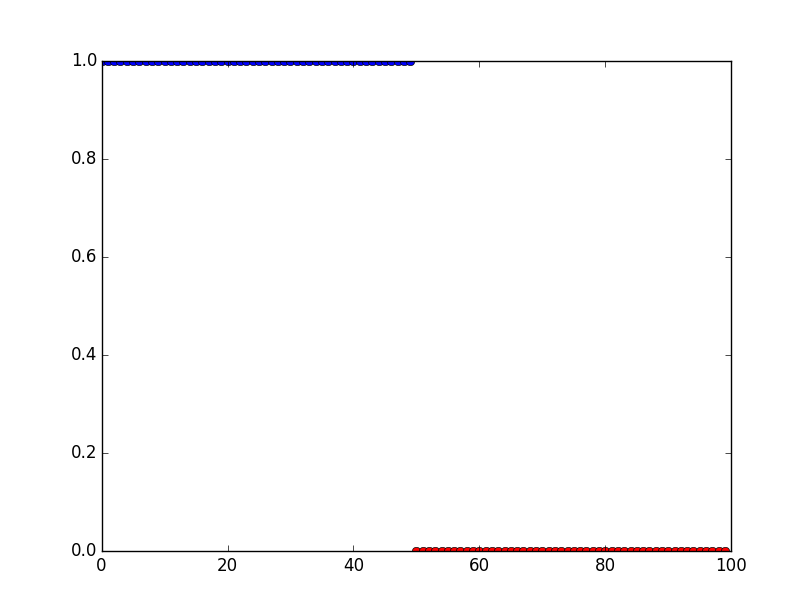
\includegraphics[scale=0.5]{classify.png}
	\caption{Classification Result}
	\label{fig3}	
\end{figure}
\end{document}



